\documentclass[main.tex]{subfiles}
\begin{document}

\section{Introduction}
This project seeks to provide means for translating from a subset of English
into Overpass queries using Combinatory Categorial Grammar.

\subsection{Motivation}
It is often the case that humans need to communicate a concrete question
or order (a query) to a computer. The most straight-forward way for this to happen is
to make the human write out their query in a domain-specific language (DSL),
specially crafted to handle the given type of query. This approach, albeit
very efficient when done correctly, requires substantial upfront effort:
the human needs to get familliar with the DSL and must have access to a specific
medium (usually a keyboard and a screen). Thus, in some cases, it is desirable
to form an expression in a natural language (or a language very similar to a
subset of a natural language) and have it translated to a query in the given
DSL.

The point is not to translate \emph{any} sentance in the source language
which has semantics applicable to the target DSL, but rather to define a
subset of the source language, in which a human could express a query
reasonably easily.

Most DSLs have compositional semantics, which makes them a great candidate
for generation using Combinatory Category Grammar (CCG) \cite[p.~181]{nts}.

One such DSL is the Overpass language, used by the open source project
OpenStreetMap for making queries to the map database. It has been chosen as
a concrete target language for this project, in order to assess the usefullness
of CCG for translating from a natural language subset to a compositional
DSL.

\begin{greenbox}
    These informal green boxes shall point out and explain lies in the formal text.

    \vspace{2mm}
    So, here goes: \emph{this section is a lie}. The actual motivation for this project
    is "The author really wanted a frendlier way to enter Overpass queries,
    and had recently learned about CCGs. So he wrote it."
\end{greenbox}

\subsection{Architecture}
The system consists of several parts:

\begin{figure}[htbp!]
    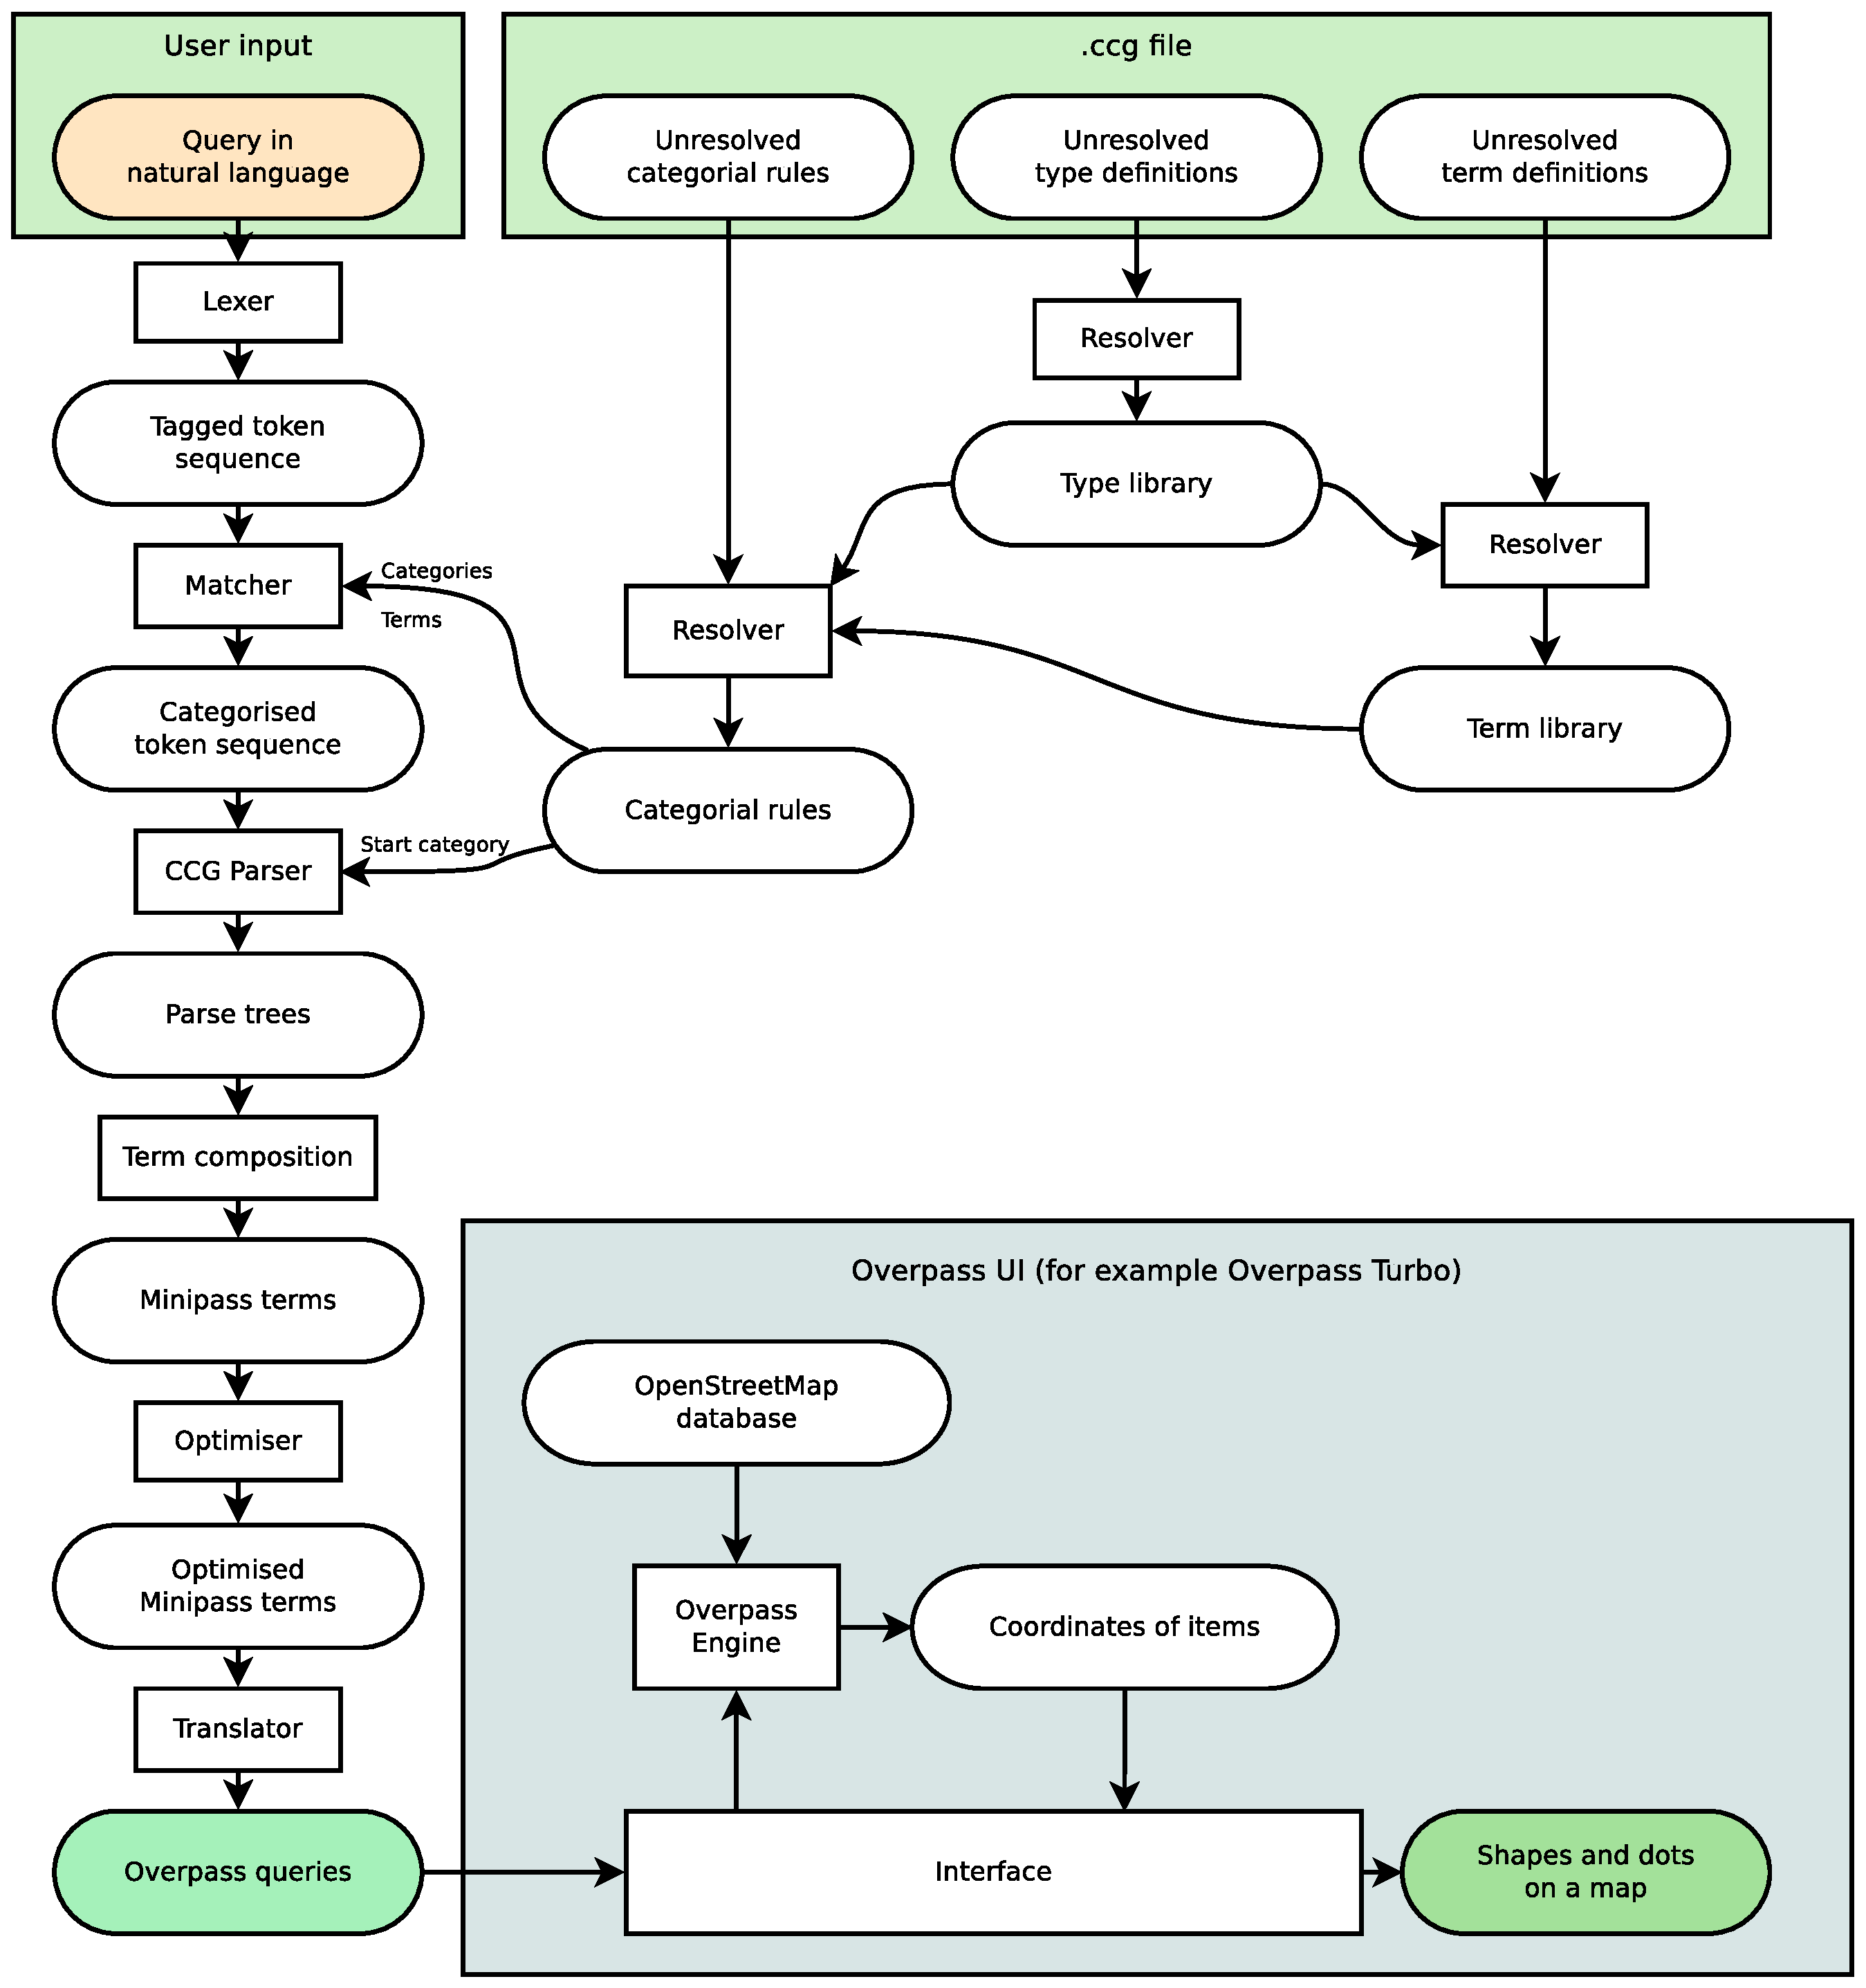
\includegraphics[width=\textwidth]{arch.eps}
    \caption{Architecture overview}
    \label{arch}
\end{figure}

\begin{itemize}
    \item Generic CCG definition language: a language for defining CCGs and
          their respective type systems and term libraries. Can be used
          standalone (for specifying CCGs which output raw parse trees)
          or by embedding a lambda calculus-based language (for specifying
          CCGs which output lambda terms)

    \item CCG Rule Matcher: a module which tags tokens from the input stream
          with Categories based on the CCG rules (defined in the CCG definition
          language)

    \item CCG Parser: a simple proof-of-concept parser based on the CYK
          algorithm

    \item English Lexer: a tokeniser, POS-tagger and lemmatiser for English
          (largely consists of external components)

    \item The Minipass language: a small, lambda calculus-based language
          which translates to Overpass, designed to be easily generated and
          to represent Overpass operators as operations on a graph.

    \item Minipass to Overpass translator: a translator from Minipass terms
          to Overpass queries which does some basic optimisations
\end{itemize}

An architecture overview can be seen at Figure \ref{arch}.


\end{document}
